\documentclass[14pt, a4paper]{extarticle}
\usepackage[T2A]{fontenc}
\usepackage[utf8]{inputenc}
\usepackage[russian]{babel}
\usepackage[paper=portrait,pagesize]{typearea}
\usepackage{graphicx}
\usepackage{lastpage}

\begin{document}
	\pagenumbering{gobble}
	\begin{center}
		Министерство образования и науки Российской Федерации\\
		Федеральное государственное бюджетное образовательное учреждение высшего образования\\
		Волгоградский государственный технический университет\\
		Кафедра <<Системы автоматизированного проектирования и поискового конструирования>>
	\end{center}
	\vspace{70pt}
	\begin{flushright}
		УТВЕРЖДАЮ\\
		Зав. кафедрой САПР и ПК\\
		\rule{25mm}{0.4pt} д.т.н. Щербаков М. В.\\
		<<\rule{7mm}{0.4pt}>> \rule{35mm}{0.4pt} 2018 г
	\end{flushright}
	
	\begin{center}
		\Large Разработка программы для автоматизации процедуры списания выпускных квалификационных работ\\
		\vspace{30pt}
		\normalsize ТЕХНИЧЕСКОЕ ЗАДАНИЕ\\
		Листов - \pageref{LastPage}\\
	\end{center}

	\vspace{70pt}
	\begin{flushright}
		Выполнили\\
		Студенты группы САПР-1.1п\\
		Верещак Г.А.\\
		Харитонов А.А.
	\end{flushright}
	
	\vspace*{\fill}
	\begin{center}
		Волгоград, 2018г.\\
	\end{center}
	\newpage
	
	\pagenumbering{arabic}
	\setcounter{page}{2}
	\tableofcontents
	\newpage
	
	\section{Введение}
	\subsection{Наименование программы}
	Наименование – «Программа для автоматизации процедуры списания выпускных квалификационных работ (ВКР)». \\Краткое наименование – программа.
	\subsection{Краткая характеристика области применения}
	Разрабатываемая программа предназначена для применения на кафедре САПР и ПК ВолгГТУ и должна служить эффективным инструментом для для списания ВКР.
	
	\section{Основания для разработки}
	\subsection{Документы, на основе которых ведётся проектирование}
	В качестве лабораторной работы №4 по курсу «Проектирование АСОиУ» было получено задание на проектирование программы, автоматизирующей процедуру списания ВКР.
	\subsection{Организация, утвердившая документ, и дата утверждения}
	Документ утвердил д.т.н., зав. кафедрой САПР и ПК Щербаков М. В.\\
	Дата утверждения документа: <<\rule{7mm}{0.4pt}>> \rule{35mm}{0.4pt} 2018 г
	\subsection{Наименование темы разработки}
	Тема разработки – «Разработка программы для автоматизации процедуры списания выпускных квалификационных работ».
	
	\section{Назначение разработки}
	Разрабатываемая программа предназначена для формирования описи по списываемым ВКР.
	
	\section{Требования к программе}
	\subsection{Требования к функциональным характеристикам}
	\subsubsection{Требования к составу выполняемых функций}
	Программа должна обеспечивать конечному пользователю возможность выполнения перечисленных ниже функций:
	\begin{itemize}
		\item получение приказов по утверждению тем ВКР;
		\item получение приказов по отчислению;
		\item получение ФИО студентов и соответствующих тем ВКР посредством парсинга таблицы с темами и ФИО студентов в приказах по утверждению ВКР;
		\item получение информации об отчислениях посредством парсинга документов с приказами об отчислениях;
		\item формирование таблицы с приказами по утверждению тем ВКР в программе;
		\item формирование таблицы с приказами по отчислению в программе;
		\item формирование шаблона описи для списания ВКР;
		\item автоматическое заполнение полей "ФИО студента" и "Тема работы" в описи на основе данных, извлеченных из приказов по утверждению тем ВКР и из приказов по отчислениям;
		\item заполнение полей описи "Количество листов ПЗ" и "Примечания";
		\item редактирование записей описи.
		
	\end{itemize}
	
	\subsubsection{Требования к организации входных данных}
	На вход программы должны быть переданы следующие входные данные.
	\begin{itemize}
		\item информация о приказах по утверждению тем ВКР должна подаваться на вход программы в виде электронной таблицы в документе в формате .docx;
		\item информация о приказах по отчислениям должна подаваться на вход программы в виде документа в формате .docx;
		\item форма описи должна быть представлена в виде документа в формате .docx;
		\item количество листов пояснительной записки в форме описи указываются в виде числа;
		\item примечания в форме описи задаются в виде текстовой строки.
	\end{itemize}
	
	\subsubsection{Требования к организации выходных данных}
	Выходные данные должны быть представлены сформированной описью в формате .docx.
	
	\subsection{Требования к надёжности}
	\subsubsection{Требования к обеспечению надёжного функционирования программы}
	Надежное функционирование программы должно быть обеспечено совокупностью организационно-технических мероприятий, перечень которых приведен ниже:
	\begin{itemize}
		\item организацией бесперебойного питания технических средств;
		\item использованием лицензионного программного обеспечения.
	\end{itemize}
	
	\subsubsection{Время восстановления после отказа}
	Время восстановления после отказа, вызванного сбоем электропитания технических средств (иными внешними факторами), не фатальным сбоем (не крахом) операционной системы, не должно превышать времени, требуемого на восстановление подачи электропитания и запуск программы.\\
	Время восстановления после отказа, вызванного неисправностью технических средств, фатальным сбоем (крахом) операционной системы, не должно превышать времени, требуемого на устранение неисправностей технических средств, и переустановки программных средств.
	
	\subsubsection{Отказы из-за некорректных действий оператора}
	Отказы программы возможны вследствие некорректных действий оператора (пользователя) при взаимодействии с операционной системой. Во избежание возникновения отказов программы по указанной выше причине следует обеспечить работу конечного пользователя без предоставления ему административных привилегий.
	
	\subsection{Условия эксплуатации}
	\subsubsection{Требования к численности и квалификации персонала}
	Минимальное количество персонала, требуемого для работы программы должно не менее 2 штатных единиц – системный администратор и конечный пользователь программы.\\
	Системный администратор должен иметь высшее профильное образование и сертификаты компании-производителя операционной системы. В перечень задач, выполняемых системным администратором, должны входить:
	\begin{itemize}
		\item задача поддержания работоспособности технических средств;
		\item задачи установки (инсталляции) и поддержания работоспособности системных программных средств – операционной системы.
	\end{itemize}

	\subsection{Требования к составу и параметрам технических средств}
	Состав технических средств, а также общесистемного и прикладного программного обеспечения программы:
	\begin{itemize}
		\item операционная система Microsoft Windows XP и старше;
		\item процессор Intel Pentium 4 или AMD Athlon с тактовой частотой выше 1.4 ГГц;
		\item ПЗУ на 1Гб;
		\item объем свободной оперативной памяти – 1 Гб;
		\item видеоадаптер SVGA, монитор, поддерживающий режим работы SVGA;
		\item клавиатура, мышь.
	\end{itemize}

	\subsection{Требования к информационной и программной совместимости}
	\subsubsection{Требования к методам решения}
	
	Данные методы решения должны обеспечивать выполнение всех этапов проектирования программы в соответствии с их порядком и сроками выполнения, указанными в разделе 6 данного документа.
	\subsubsection{Требования к исходным кодам и языкам программирования}
	Исходные коды программы должны быть реализованы на языке 1C версии 8.2. В качестве интегрированной разработки должна быть использована среда 1C Конфигуратор.
	
	\subsection{Требования к программным средствам, используемым программой}
	Системные программные средства, используемые разрабатываемой программой, должны быть представлены лицензионной локализованной версией операционной системы, а также платформой 1с.
	
	\section{Требования к программной документации}
	\subsection{Состав программной документации}
	Состав программной документации должен включать в себя техническое задание на разработку и проектирование программы (ГОСТ 19), пояснительную записку, руководство пользователя и исходные коды программы.
	
	\section{Стадии и этапы разработки}
	Проектирование программы должно включать в себя стадии, приведённые в Таблице 1.\\
	\begin{table}[h!]
		\caption{Сроки выполнения работ}
		\begin{center}
			\label{tab:table1}
			\begin{tabular}{|c|c|c|}
				\hline
				№ п/п & Наименование стадии             & Сроки         \\
				\hline
				1     & Анализ требований пользователя  & 20/11/2018     \\
				\hline
				2     & Разработка технического задания & 22/12/2018     \\
				\hline
			\end{tabular}
		\end{center}
	\end{table}
	
	\section{Порядок контроля и приёмки}
	\subsection{Виды испытаний}
	Приёмо-сдаточные испытания должны проводиться не ранее окончания реализации программного продукта.
	\subsection{Общие требования к приёмке работы}
	Возможность приёмки программы должна определяться соответствием всем пунктам настоящего технического задания.
	
	\newpage
	\section*{Приложение А. BPMN-диаграмма автоматизируемого процесса}
	\addcontentsline{toc}{section}{Приложение А. BPMN-диаграмма автоматизируемого процесса}
	% bpmn-diagram.png
	\begin{figure}[h!]
		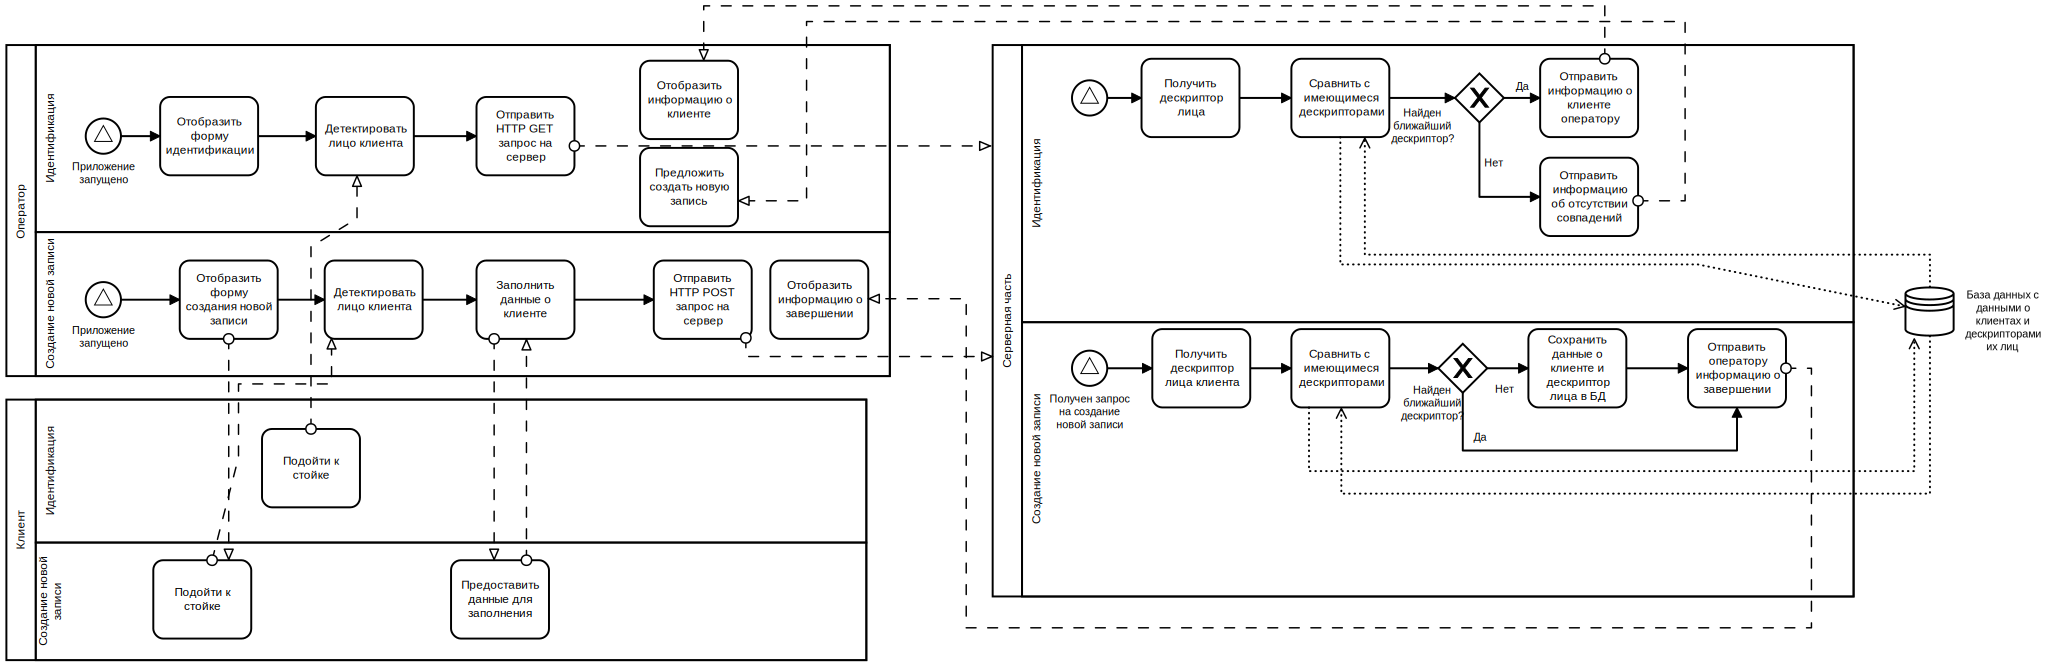
\includegraphics[width=\linewidth]{diagram.png}
		\caption{BPMN-диаграмма автоматизируемого процесса}
		\label{fig:diagram1}
	\end{figure}

	\newpage
	\section*{Приложение Б. Шаблон описи}
	\addcontentsline{toc}{section}{Приложение Б. Шаблон описи}
	% bpmn-diagram.png
	\begin{figure}[h!]
	\includegraphics[width=\linewidth]{diagram2.png}
	\caption{Шаблон описи}
	\label{fig:diagram2}
	\end{figure}
	
\end{document}